As described in section \ref{stressnstrain} Cauchy’s strain tensor is only valid for small deformations. This is a problem since only large deformations result in visually interesting effects. In section \ref{eqn:stiffnessmatrix} the stiffness matrix is obtained from $V_{e}$, $B_{e}$ and $E$ which are all constant depending on the initial state of the tetrahedron. Due to large deformations during simulation time this stiffness matrix will become unvalued. M\"uller \cite{muller_ivm} proposed a solution to this problem called Stiffness Warping. This method compensates the error by rotating the deformed tetrahedron back into its original coordinate frame. The rotation is found by forming the matrix A which is the non translation part of the mapping between the two tetrahedrons shown in equation.

\begin{equation}\label{eqn:mappedTetraMatrix}
    \mathbf{A} = [\mathbf{x}_{1}-\mathbf{x}_{0}, \mathbf{x}_{2}-\mathbf{x}_{0}, \mathbf{x}_{3}-\mathbf{x}_{0}][\mathbf{p}_{1}-\mathbf{p}_{0}, \mathbf{p}_{2}-\mathbf{p}_{0}, \mathbf{p}_{3}-\mathbf{p}_{0}]^{-1}
\end{equation}

A Gram-Schmidt method is used to extract the rotation matrix $\mathbf{R}$  from matrix $\mathbf{A}$ , there are several other ways of doing this procedure, however this one is quite simple and works good for this application. As described in \cite{rt_phys} $\mathbf{A}$ the is in the following form

\begin{equation}\label{eqn:transformationAxes}
    A =[\mathbf{a}_0, \mathbf{a}_1,\mathbf{a}_2]
\end{equation}

Where $\mathbf{a}_i$ are the axes of the transformation described in equation \ref{eqn:mappedTetraMatrix}. Note that it is important to ensure that these are normalized and orthogonal to eachother. The three columns of the rotation matrix are finally computed by using the Gram-Schmidt method as follows

\begin{equation}\label{eqn:r0}
    \mathbf{r}_0 = \frac{\mathbf{a}_0}{| \mathbf{a}_0 |}
\end{equation}

\begin{equation}\label{eqn:r1}
    \mathbf{r}_1 = \frac{\mathbf{a}_1 -  \mathbf{r}_0 \cdot \mathbf{a}_1}{| \mathbf{a}_1 -  \mathbf{r}_0 \cdot \mathbf{a}_1 |}
\end{equation}

\begin{equation}\label{eqn:r2}
    \mathbf{r}_2 =  \mathbf{r}_0 \times  \mathbf{r}_1
\end{equation}

The rotation matrix is then assembled as $\mathbf{R}_e =[ \mathbf{r}_0 ,  \mathbf{r}_1 ,  \mathbf{r}_2]$. It should be noted that $\mathbf{r}_2$ is not computed using the Gram-Schmidth method but is instead the cross product of $\mathbf{r}_0$ and  $\mathbf{r}_1$ to ensure a right handed system.

Now that the rotational part $\mathbf{R}_e$ is extracted from the deformation it can be used to rotate the deformed vertices $\mathbf{x}$ back to their non-rotated state $\mathbf{R}_e^{-1} \mathbf{x}$. By multiplying the displacements in this state with the stiffness matrix $\mathbf{K}_e$ the linear forces $\mathbf{K}_e (\mathbf{R}_e^{-1} \mathbf{x} - \mathbf{x}_0)$ is achieved. These forces are then finally rotated back to the actual deformed state as follows

\begin{equation}\label{eqn:f_warped}
     \mathbf{f}_{warped} = \mathbf{R}_e \mathbf{K}_e (\mathbf{R}_e^{-1} \mathbf{x} - \mathbf{x}_0)
\end{equation}

With this new inner force the global stiffness matrix $\mathbf{K}$ have to be constructed a bit differently by assembling it with $\mathbf{K}'_e = \mathbf{R}_e \mathbf{K}_e \mathbf{R}_e^T$ instead of only $\mathbf{K}_e$. And the implicit euler equation \ref{eqn:impEuler} has to be rewritten as

\begin{equation}\label{eqn:warpedImpEuler}
		(\mathbf{M} + \Delta t  \mathbf{C} + \Delta t^2 \mathbf{K})v^{t+1} = \mathbf{M} v - \Delta t (\mathbf{Kx}-\mathbf{f}_0 + \mathbf{f}_{ext})
\end{equation}

Where 

\begin{equation}\label{eqn:f0}
		\mathbf{f}_0 = \mathbf{R}_e \mathbf{K}_e \mathbf{x}_0
\end{equation}



\begin{figure}[h]
\centering
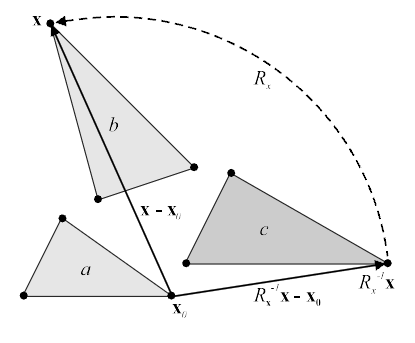
\includegraphics[width=.5\columnwidth]{figures/warpedstiffness.png}
\caption{}
\label{fig:4}
\end{figure}